\scanpage{114}
\margin{\figure{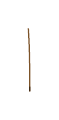
\begin{tikzpicture}
\draw[brown!65!black,line width=.45pt] (0,0) .. controls (.015,-.20) and (.02,-.55) .. (.02,-.80);
\draw[brown!35!black,line width=.45pt] (.019,-.74)--(.02,-.80);
\end{tikzpicture}}}
est de plus propre, alors pour \uline{toute} sous-variété linéaire $\inserted{L_t}$ de codimensio\handwritten{n} $s$, $Y_t=f_t^{-1}(L_t)$ est géométriquement connexe.

Conjuguant avec 2, on trouve, par l'argument qui a permis de déduire 3 de 1 :

\margin{\handwritten{\begin{tabular}{@{}l@{}}cf.\\S\unsure{C|G}A 1 X \unsure{2,11|2.11|2,II|2.II}\end{tabular}}}
\margin{\figure{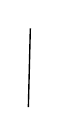
\begin{tikzpicture}
\draw[black,line width=.5pt] (.025,0)--(0,-1);
\end{tikzpicture}}}
\uline{Corollaire} 5: \deleted{Avec}\inserted{\handwritten{Sous}} les hypothèses de \unsure{3|4} , \inserted{avec $X$ propre,} l'homomorphisme danonique $\handwritten{\pi}_1(Y_{\bar t})\handwritten{\rightarrow}\handwritten{\pi}_1(X)$ ($\handwritten{\simeq}\handwritten{\pi}_1(X_{\bar t})$ par le théorème de changement de base) est surjectif.

Nous désirons également un énoncé analogue à 5, donnant une surjectivité pour des $\handwritten{\pi}_1$ pour un $t$ non générique, mais sans hypothèse de propreté, et pour des quotients plus gros du $\handwritten{\pi}_1$ que ceux envisagés dans (**). On peut\deleted{\unsure{nt|on}} donner à ce sujet le résultat suivant:

\margin{\figure{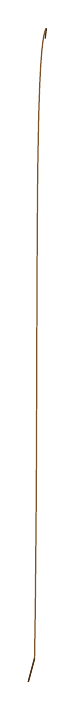
\begin{tikzpicture}
\draw[brown!65!black,line width=.45pt] (.15,0) .. controls (-.02,-.2) and (.06,-4) .. (0,-8) --(-.08,-8.3);
\draw[brown!35!black,line width=.45pt] (.15,0)--(.135,-.13);
\draw[brown!35!black,line width=.45pt] (0,-8)--(-.08,-8.3);
\end{tikzpicture}}}
\uline{Théorème} 6. Su\unsure{p|i}\unsure{p|t}osons $k$ algébriquement clos, \inserted{\handwritten{et}} $X$ propre, $f:X\handwritten{\rightarrow}P^r$, \deleted{et} le sous -espace linéaire $L_t$ de $P^r$ de codimension $s$ (défini sur $k$, pour fixer les idées) \deleted{tels qu'on ait} et enfin le sous-schéma fermé $D$ de $X$ tels qu'on ait ceci; \deleted{où on a posé $U=X-D$}

a) \deleted{$U_t=U\unsure{\cap}X_t$ et} $\deleted{X}\handwritten{Y}_t=f^{-1}(L_t)$ est non vide.

b) Pour tout $x\handwritten{\in}\deleted{X}\handwritten{Y}_t$, $X$ est lisse en $x$, $Y_t$ est lisse en $x$\handwritten{,} de codi\unsure{memt|ment|mem|men}sion $s$ dans $X$ en $x$, $f$ est net en $x$.

c) Pour tout $x\handwritten{\in}D_t=D\handwritten{\cap}Y_t$, o\deleted{\unsure{\`{}}}u \deleted{bien} bien $\operatorname{codim}_x(D_t,\underset{\begin{tikzpicture}[x=1mm,y=1mm,baseline]
\fill[black] (-.40,.45) ellipse (.10 and .14);
\fill[brown!35!black] (-.64,0) ellipse (.11 and .11);
\end{tikzpicture}}{\deleted{\unsure{T|X}}\handwritten{Y}}_t)\handwritten{\geqslant}2$, ou bien $D_{\deleted{\unsure{t}}}$ est un diviseur \unsure{e|s}\unsure{n|u}r $X$ en $x$ et $\deleted{D_t}$ induit sur $Y_t$ en $x$ un diviseur à croisements normaux.

Supposons $U=X-D$ irréductible, et considérons l'inclusion $U_t=U\handwritten{\cap}Y_t\handwritten{\longrightarrow}U$ . \deleted{Alors $U_t$} Soit $\handwritten{\pi}_1^t(U)$ le \deleted{\unsure{grou|gros}} quotient du groupe fondamental de $U$ \deleted{formé des} qui classifie les revêtements de $U$ qui sont modérément ramifiés en les composantes irréductibles de codimension 1 de $D$ dans $X$ qui rencontrent $Y_t$, \deleted{(\unsure{i.e.} telles que $D$} et $\overset{\unsure{t}}{\handwritten{\pi}}_1^t(\unsure{U|V}_t)$ le quotient \deleted{analogue} de $\handwritten{\pi}_1(U_t)$ qui classifie les revêtements qui sont modérément ramifiés en les composantes irréductibles de codimension 1 de $D_t$ . On a un homomor-
% archive sheet number: 113

